% -*- mode: LaTeX; coding: utf-8; -*-

\chapter{Katsaus yleisimpiin hyökkäyksiin}
Nykyisin yksikään verkossa oleva kone ei ole suojassa tietoturvahyökkäyksiltä,
ja niiden aiheuttamilta ongelmilta. Näitä hyökkäyksiä on hyvin monenlaisia, ja
ne voidaan jakaa eri kategorioihin niiden tavoitteiden ja toteutustapojen
mukaan. Uusia hyökkäystapoja myös kehitetään jatkuvasti, ja vanhat saavat uusia
ominaisuuksia. Vaikka osaan hyökkäyksistä onkin olemassa suojautumistapoja, on
näiltä kaikilta suojautuminen ylläpitäjälle mahdoton tehtävä. Verkon
turvallisuuden kannalta on kuitenkin tärkeää, että näiden tuomat riskit
tiedostetaan ja niihin pyritään puuttumaan mahdollisuuksien ja resurssien
mukaan.

\section{Tiedon urkinta ja väärentäminen}

Ennen kuin hyökkääjä pystyy murtautumaan verkkoon tai koneeseen, tulee hänen
selvittää kohteen mahdolliset heikkoudet. Haluttuja tietoja ovat mm. mitä
käyttöjärjestelmiä koneisiin on asennettu, mitkä versiot ohjelmistoista on
käytössä ja mikä on verkon rakenne ja tietoturvataso. Näiden tietojen
selvittämiseksi hyökkääjää aloittaa verkkoa kohtaan joukon hyökkäyksiä, joita
kutsutaan tiedusteluhyökkäyksiksi. (engl. Probe Attacks). Kyseiset hyökkäykset
ovat hyökkäyksistä yleisimpiä, sillä niiden toteuttaminen ei vaadi hyökkääjältä
usein kovinkaan syvällistä osaamista. Verkosta löytyy paljon valmiita työkaluja,
joiden avulla hyökkääjä pystyy urkkimaan tarvittavat tiedot sekä mahdol-lisesti
saman tien hyödyntämään löydettyjä heikkouksia. Hyökkääjä, jolla on tarkka
kuvaus verkon laitteista ja palveluista, voikin käyttää tietoa
haavoittuvuuksien etsimiseen ja järjestelmiin murtau-tumiseen [8].

Kun hyökkääjällä on tietämys verkon eri komponenteista, voi hän aloittaa
hyökkäysten suunnittelun. Yksi tapa pyrkiä murtautumaan IP-pohjaiseen verkkoon
on hyödyntää protokollissa olevia heikkouksia. Tällaisia hyökkäyksiä kutsutaan
spoofing-hyökkäyksiksi, ja niissä hakkeri pyrkii naamioimaan oman koneensa
siten, että se näyttäisi kuuluvan kohteena olevan koneen kanssa samaan verkkoon.
Tällöin hyökkääjä pystyy huijaamaan kohdekonetta jakamaan ja lähettämään
arkaluontoista dataa, jota muuten vain jaettaisiin luotettujen kohteiden kesken.
Hyökkäykset jaotellaan edelleen sokeisiin ja aktiivisiin hyökkäyksiin. Nämä
eroavat siinä, että sokeassa hyökkäyksessä murtautujalla ei ole tarkkaa tietoa
sen koneen IP:stä, jota hän yrittää esittää tai koneelta puuttuu tarvittavat
oikeudet. Tällöin hyökkääjä joutuu tekemään hyökkäykset sokeana. Aktiivisessa
hyökkäyksessä murtautujalla taas on tieto koneiden välisistä oikeuksista,
jolloin tiedon korruptoiminen, muokkaaminen ja välittäminen toiseen verkkoon
ovat mahdollista [7].

\subsection{IP Spoofing}

IP Spoofing on hyökkäystapa, jossa hyökkääjä pyrkii murtautumaan verkkoon
käyttäen luotetun koneen IP:tä. Ensimmäisessä vaiheessa hyökkääjän selvittää
luotetun kohteen IP:een käyttäen joko sokeaa tai aktiivistä hyökkäystapaa.
Varsinainen hyökkäys tapahtuu, kun kohdekone yrittää muodostaa yhteyden
koneeseen, jonka IP:een hakkeri on ottanut käyttöönsä. Tässä onnistuakseen
hakkerin tulee ylläpitää tietoa luotetun koneen käyttämistä TCP:een
kuittausnumeroista, joita käytetään kolmivaiheisessa yhteydenmuodostuksessa.
Tämän tiedon avulla hakkeri pystyy muokkaamaan yhteyden vaatimia
kuittausviestejä siten, että ne sisältävät oikeat kuittausnumerot. Nämä
kuittausnumerot hyökkääjä joutuu aluksi usein arvaamaan, jonka takia tämä
hyökkäystapa on monimutkainen toteuttaa [7].

\begin{figure}[ht]
\centering
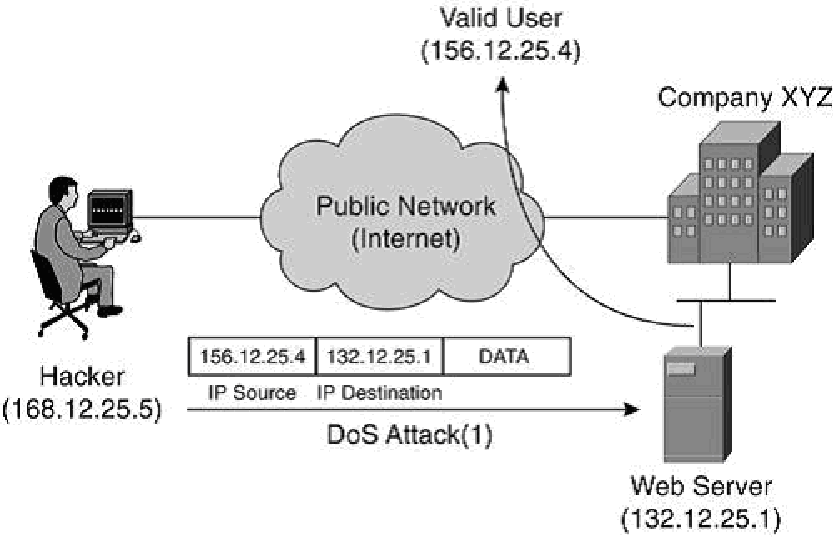
\includegraphics[width=10cm]{pics/spoofing.pdf}
\caption[Conventional electrode positioning]{Conventional 10--20 electrode positions. Figure adapted from Sanei and Chambers}
\label{ELECTRODE_POSITIONS}
\end{figure}

Vaikka IP spoofing hyökkäykset ovat vaikeita toteuttaa, ovat ne melko yleisiä,
koska jokainen TCP/IP protokollaa käyttävä järjestelmä on sille altis. Tämä
johtuu siitä, että TCP/IP-pino sallii pakettien käsin muokkaamisen. Tämä
toiminto on sallittu, koska toimiakseen jotkut IP-pohjaiset palvelut joutuvat
käsin muokkaamaan pakettien sisältöä ennen lähettämistä. Tällaisia palveluita
ovat mm. mobiili IP-ympäristö ja VPN-järjestelmät, joissa lähettäjän IP
muutetaan toiseksi [11].

IP spoofing hyökkäyksiä voidaan torjua monin eri keinoin. Tehokkain tapa on
asettaa verkko siten, että se ei salli sellaisten pakettien kulkua, jotka
väittävät kuuluvansa sisäverkon koneelle, mutta jotka tulee verkkoon
ulkopuolisesta liitännästä. Jos tämä kuitenkin halutaan sallia, niin jokainen
sessio tulisi kryptata reitittimessä. Muutenkin yhteyksien muodostumisen tulisi
pohjautua koko järjestelmän kattavaan salaukseen [7].

\section{Denial Of Service}

Yksi tietoturva-alan johtavista tutkimuskeskuksista CERT [1]
määrittelee palvelunestohyökkäyksen (engl. Denial of Service)
sellaiseksi teoksi, jossa hyökkääjän tavoitteena on estää laillisia
käyttäjiä käyttämästä heille kuuluvia/käytössä olevia
palveluita. Tällaisia palveluita voivat olla esimerkiksi verkon
resurssien käyttö sekä verkon yli käytettävät
web-sovellukset. Hyökkäyksillä pyritään lamauttamaan palvelua tarjoava
verkko tai palvelin siten, että oikeiden pyyntöjen vastaanottamiseen
ei enää riitä resursseja. Keinoja tähän on monia, ja koska näistä
lähes jokainen käyttää nykyisin hyväkseen eri protokollien sallittuja
toimintoja, on hyökkäyksiä vastaan suojautuminen hyvin vaikeaa [2].

Palvelunestohyökkäykset voidaan jakaa kolmeen ryhmään näiden
toteutustapojen ja tavoitteiden mukaan. Ensimmäiseen ryhmään kuuluvat
hyökkäykset, joiden tarkoitus on rajoitettujen resurssien loppuun
kuluttaminen. Tämä voidaan toteuttaa esimerkiksi kuormittamalla verkko
tai palvelin turhilla pyynnöillä. Toiseen ryhmään kuuluvat
hyökkäykset, jotka pyrkivät joko tuhoamaan tai muuttamaan
konfigurointitietoja siten, että kone tai verkko ei toimi enää
ollenkaan. Viimeiseen ryhmään kuuluvat verkon komponenttien
muokkaamiseen tai tuhoamiseen tähtäävät hyökkäykset [1]. Vaikka tässä
työssä keskitytään vain resursseihin kohdistuviin hyökkäyksiin, niin
palvelun kokonaisturvallisuuden kannalta jokaiseen ryhmään tulee
yrityksessä kiinnittää tasapuolisesti huomiota.

Vielä viime vuosikymmenellä palvelunestohyökkäykset perustuivat
yleensä käyttöjärjestelmistä löydettyjen heikkouksien
hyödyntämiseen. Näiden hyökkäysten aikaansaama tuho oli usein
konekohtaista ja melko rajattua, joten hyökkäyksiä ei nähty kovinkaan
vakavana uhkana. 2000-luvulla palvelunestohyökkäykset ovat kuitenkin
kehittyneet siihen pisteeseen, että nykyisin palvelu saattaa joutua
hajautetun palvelunestohyökkäyksen (engl. Distrubuted Denial of
Service) kohteeksi, jolloin palvelua saattaa olla lamauttamassa jopa
yli 140000 saastunutta konetta. Tällaisia saastuneita koneita
kutsutaan zombeiksi, sillä näihin on murtauduttu ja asennettu
ohjelmisto, jonka avulla murtautuja pystyy hallitsemaan konetta
käyttäjän tietämättä. Zombie-verkoston ei tarvitse edes olla kovinkaan
suuri aiheuttaakseen tuhoa, sillä jo 3000 koneen verkosto, jossa
jokainen kone tuottaa 25 Kbps liikennettä, aiheuttaa yhteensä 75 Mbps
kuorman verkolle [2]. Palvelunestohyökkäyksen seuraamukset
saattavatkin olla varautumattomalle taholle usein katastrofaaliset, ja
pahimmillaan hyökkäys saattaa pysäyttää organisaation toiminnan
useiksi päiviksi [1].

Viime vuosina palvelunestohyökkäykset ovat edelleen kehittyneet
käsittämään verkkokerroksen raa’an voiman hyökkäysten lisäksi myös
sovelluskerroksen hyökkäykset, joiden toteuttaminen vaatii usein
hyökkääjältä vain vähän resursseja [2]. Nämä sovelluskerroksen
hyökkäykset ovat toteutukseltaan usein hyvin hienostuneita, ja ne
jäävät yleensä huomaamatta yrityksen tietoturvaratkaisuilta, koska ne
eivät poikkea normaalista liikenteestä. Hyökkääjä saattaa esimerkiksi
pyytää sellaista resurssia palvelulta, jonka pyytäminen vie vain vähän
hyökkääjän omia resursseja, mutta aiheuttaa palvelimelle suuren
kuorman [3]. Tällaisen hyökkäyksen teho nähtiin jo vuonna 2004, kun
MyDoom-viruksella saastuneet koneet kuormittivat suuresti yleisimpiä
hakukoneita etsimällä näiden avulla uusia sähköpostiosoitteita, joihin
lähettää saastunut sähköposti [2]. Sovelluskerroksen hyökkäyksen
vaikutus voidaan kohdistaa myös haluttua palvelua kohti, jolloin
vaikutukset ovat vieläkin suuremmat. Näin tapahtui, kun Yhdysvalloissa
yrittäjä palkkasi ”DDoS mafian” kaatamaan kilpailijoidensa nettisivut
HTTP-kutsuilla, jotka pyysivät ladattavaksi isoa kuvatiedostoa
[3]. Tämä aiheutti kolmelle kilpailijalle arviolta jopa yhden
miljoonan dollarin tappiot, ja pysäytti toiminnan lähes kahdeksi
viikoksi [4].

\subsection{SYN-hukuttaminen}

TCP/IP-protokollan yksi suunnittelulähtökodista oli, että sitä
käytettäisiin avoimessa ja luotetussa ympäristössä. Tästä syystä sen
suunnittelussa ei osattu ottaa huomioon mahdollisia vihamielisiä
käyttäjiä, jotka pyrkisivät häiritsemään muita käyttäjiä sen
avulla. TCP/IP-protokollan käyttö kuitenkin levisi ja yleistyi
arvaamattomasti, jonka johdosta suunnitteluvaiheessa tehdyt virheet
periytyivät nyt käytössä olevaan IPv4-verkkorakenteeseen[2].

Perityistä heikkouksista tunnetuin ja käytetyin lienee
SYN-hukuttamiseksi kutsuttu hyökkäys, jossa hyökkääjä pyrkii
kuluttamaan kohteen kaistan loppuun tekaistuilla
yhteydenmuodostuspyynnöillä. Hyökkäys on toteutukseltaan hyvin
yksinkertainen ja helppo toteuttaa, sillä se käyttää hyväkseen
TCP-protokollaan määritettyjä toimintoja. Hyökkäys perustuu siihen,
että kolmiosaisessa yhteydenmuodostusvaiheessa kone lähettää
palvelimelle SYN-paketin, jonka johdosta palvelin varaa tulevalle
yhteydelle resursseja ja lähettämänsä SYN/ACK-viestin jälkeen jää
odottamaan yhteyden muodostamista. Tähän koneen kuuluu vastata
ACK-viestillä, jonka jälkeen yhteys muodostetaan [2].

Tähän toimintamalliin perustuu mm. HTTP-protokollan toiminta, ja sen
avulla web-palvelimet pystyvät nopeasti palvelemaan käyttäjiä. Koska
TCP-protokolla pyrkii aina varmistamaan yhteyden muodostumisen, ja
tarvittaessa lähettämään SYN/ACK-viestin uudestaan SYN-paketin
lähettäneelle koneelle, pystyy hyökkääjä käyttämään tätä ominaisuutta
hyväkseen. Riittää, että hyökkääjä nuuskii selville käyttämättömän
IP-osoitteen, joka on mieluiten samasta osoiteavaruudesta kuin missä
palvelin on. Tämän jälkeen hyökkääjä luo SYN-paketin, jossa on tämä
tekaistu IP-osoite. Koska palvelimen lähettämä SYN/ACK-viesti ei
koskaan saavu oikealla koneelle, ei palvelin saa ACK-kuittausta,
jolloin TCP-protokolla alkaa lähettämään pakettia uudestaan niin kauan
kunnes määritetty raja yhteyden aikakatkaisulle tulee vastaan
[6]. Hyökkääjälle riittää, että tämä toiminta automatisoidaan ja
koneina käytetään esimerkiksi jo aikaisemmin mainittuja
zombie-koneista muodostettuja verkostoja.

SYN-hukuttamisen mahdollistavan mekanismin avulla voidaan myös
toteuttaa heijastettu hyökkäys (engl. reflective attack), joka on
muunnos SYN-hukuttamisesta. Tässä hyökkäyksessä väärennetyissä
SYN-viesteissä on lähettäjäksi merkitty haluttu kohde. Lähettämällä
suuri määrä näitä SYN-viestejä esimerkiksi web-palvelimelle, aiheutuu
vastaustulvasta ongelmia kohteelle [6].

Koska harvalla yrityksellä on mahdollista pitää ylimääräisiä
resursseja SYN-hu\-kut\-ta\-mi\-sen varalta, joudutaan ratkaisua hakemaan
muilla keinoin. Yksi alkeellinen keino on rajoittaa puoliavonaisten
yhteyksien määrää, jolloin rajan ylittyessä aletaan yhteyksiä pudottaa
[5]. Toinen käytetty keino on reitittimiltä verkkoon päin tulevan
liikennemäärän seuraaminen, ja liikennepiikkeihin
reagoiminen. Hyökkäyksiä vastaan voidaan myös suojautua liikenteen
seuraamiseen tarkoitetuilla sovelluksilla sekä pääsylistoilla
[6]. Täydellistä turvaa nämä eivät kuitenkaan tarjoa, sillä hyvin
toteutettua hyökkäystä vastaan on vaikea suojautua ilman, että
sallittuja yhteyksiä ei tiputettaisi.

\subsection{UDP Echo}

Myös UDP-protokolla mahdollistaa hyökkäysten tekemisen. Nämä
hyökkäykset käyttävät hyväkseen UDP:n ECHO-toimintaa, johon muut
koneet vastaavat jollei verkossa toisin ole määritelty. Fraggleksi
nimetty hyökkäys toimii siten, että hyökkääjä lähettää UDP
echo-viestin yleislähetyksenä, johon on merkitty lähettäjäksi
hyökkäyksen kohde. Tähän viestiin kaikki verkon koneet vastaavat,
jolloin kohdekoneen kaista ja resurssit loppuvat. Fraggle on hyvä
esimerkki vahvistetusta hyökkäyksestä, jossa verkon laitteiden määrä
vaikuttaa siihen, kuinka vakava hyökkäys on [7]. Vastaavanlainen
hyökkäys voidaan myös toteuttaa kahden koneen välillä, jos kummassakin
on sallittuna UDP echo-viestit. Tällöin hyökkääjä väärentää viestiin
lähettäjän osoitteen ja halutun kohdeportin. Vastaanottaja vastaa
tähän viestiin omalla echo-viestillä, ja näin kahden koneen välille on
muodostunut ikuinen silmukka [5].

\subsection{Smurf}

Smurf on yksi ensimmäisistä vahvistetuista DoS-hyökkäyksistä, ja se
toimii lähes identtisesti Fragglen kanssa sillä erolla, että UDP:n
sijasta käytetään ICMP-protokollaa. Hyökkääjä lähettää kohteen
puolesta yleislähetyksenä verkolle ICMP ECHO-paketin, johon verkon
laitteet vastaavat, jos ECHO-viestit on sallittuja verkossa. Jo 100
konetta verkossa pystyy aiheuttamaan 14Mbps kuorman kohdekoneelle,
joten pienikin väärin konfiguroitu verkko pystyy aiheuttamaan kuorman,
jota harva linkki pystyy pitkään kestämään [2].

Jos hyökkäys on päässyt käyntiin, ei tälle ole paljoa muuta tehtävissä
kuin poistaa kohteena olevat koneet pois verkosta. Paras vastatoimi
Fragglen ja Smurffin kaltaisille hyökkäyksille onkin konfiguroida
verkon laitteet alusta asti oikein. Yleislähetysten kieltämisellä ja
ECHO-viestien tuen poistamisella verkon laitteilta pääsee jo
pitkälle. Samoin ICMP-protokollan käyttöä kannattaa verkossa rajoittaa
[2].

\section{Remote-to-Local}

Remote-to-Local (lyh. R2L) on hyökkäystyyppi, jossa hyökkääjä pyrkii
saamaan koneelle sellaiset oikeudet, joita hänellä ei muuten
olisi. Tämä tapahtuu useimmiten käyttäen hyväksi järjestelmässä olevia
heikkouksia, joiden avulla hyökkääjä pääsee verkon yli murtautumaan
koneelle [8]. Pahimmassa tapauksessa hyökkääjä saa hankittua koneelle
pääkäyttäjän oikeudet, jolloin koneen ja verkon resurssit ovat täysin
hyökkääjän käytössä.

Onnistuneet R2L hyökkäykset ovat verkon ylläpitäjien kannalta pahimpia
mahdollisia, sillä niiden mahdollistamat tuhot ja aiheuttamat
kustannukset ovat muita hyökkäyksiä huomattavasti suuremmat
[9]. Onnistunut R2L-hyökkäys saattaa myös muut verkon koneet vaaraan,
sillä usein hyökkääjä pyrkii asentamaan koneisiin ohjelmistoja, joiden
avulla hyökkääjä pystyy ottamaan koneen haltuun käyttäjän
huomaamatta. Tällä tavoin osa aikaisemmin mainituista
Zombie-verkostoista saa alkunsa.

Käytetyimmät web-palvelinohjelmistot (Apache ja IIS) vastaavat noin
85\% kaikista käytetyistä palvelinsovelluksista. Näiden kahden lisäksi
BIND-ni\-mi\-pal\-ve\-lin\-oh\-jel\-mis\-tol\-la on markkinaenemmistö. Ohjelmistojen
yleisyydestä johtuen yli puolet R2L-hyökkäyksen mahdollistavista
heikkouksista onkin löydetty näille alustoille [8]. Useat
haavoittuvaisuudet johtuvat ohjelmointivirheistä, joiden johdosta
hyökkääjä pystyy aiheuttamaan sovellukseen muistin ylivuodon
(engl. Buffer Overflow). Tämä usein kaataa sovelluksen tai saattaa sen
sellaiseen tilaan, että hyökkääjä pystyy ajamaan omia komentoja
koneella. Kattava listaus löydetyistä heikkouksista ja näiden
korjauksista löytyy osoitteesta www.cve.mitre.org/cve [10].

Tunnetuilta R2L-hyökkäyksiltä suojautuminen on hyvin yksinkertaista
sillä nykyinen trendi on, että haavoittuvuuden löytänyt taho ilmoittaa
tästä ensin sovelluksen kehittäjille, ennen kuin julkistaa
tiedon. Siksi usein korjaus haavoittuvuuteen on olemassa ennen kuin
sitä on mahdollista hyödyntää [9]. Vastuu jääkin verkon ylläpitäjälle,
että pitää käytetyt sovellukset ajan tasalla sekä päivittää
suojausjärjestelmät siten, että ne tunnistavat tällaiset
hyökkäykset. Suurin osa onnistuneista hyökkäyksistä johtuukin siitä,
että tunnettuja tietoturva-aukkoja ei ole korjattu.

\section{User-to-Root}

User-to-Root (lyh. U2R) hyökkäyksessä murtautuja pyrkii hankkimaan
koneelle pääkäyttäjän oikeudet. Tämä tapahtuu käyttäen järjestelmässä
olevia haavoittuvaisuuksia, joita ei ole paikattu. Useimmiten
hyökkäykset pohjautuvat koodausvirheisiin, jotka mahdollistavat
ylivuodon aiheuttamisen sekä odottamattomien syötteiden antamisen
[8]. Käyttäjästä pääkäyttäjäksi hyökkäys eroaa R2L hyökkäyksestä
siten, että hyökkääjällä on jo valmiiksi pääsy koneelle normaalina
käyttäjänä.

\section{Tiedon urkkiminen ja datan muokkaaminen}

Ennen kuin hyökkääjä pystyy murtautumaan verkkoon/koneeseen, tulee
hänen selvittää mitä hänellä on vastassa. Tärkeitä tietoja ovat
mm. mikä ohjelmisto ja mikä versio siitä on käytössä, mikä
käyttöjärjestelmä ja minkälaiset suojausjärjestelmät kohteella on
käytössä. Hyökkääjä, jolla on tarkka kuvaus verkon laitteista ja
palveluista, voi käyttää tätä tietoa haavoittuvuuksien etsimiseen [8].

[1] www.cert.org
[2] Hacking Exposed
[3] DDoS-Resilient …
[4] \url{http://www.fbi.gov/wanted/fugitives/cyber/echouafni_s.htm viitattu 27.10.2009}
[5] TCP/IP verkot
[6] Hack the Stack
[7] Web Security Basics
[8] A Comparative Study of Techniques for Intrusion Detection
[9] The Effect of Identifying Vulnerabilities and Patching Software on the Utility of Network Intrusion Detection
[10] www.cve.mitre.org/cve. Viitattu 29.10.2009
